% 第3章第4节：最小费用流（问题与下界平移；负费用环判据、节点势与逐弧证书；网络单纯形法；算法分析与结果检验）。

\section{最小费用流}
\label{sec:graph-min-cost-flow}

第~\ref{sec:graph-max-flow}节只问能送多少：源点送出得越多越好，货物走哪条路、花多少代价并不计较。实际调运中，各处的产量与需求往往事先给定，同一批货物可以经由不同线路到达，而各条线路的单位运价不同。这时要比较的不再是输送量，而是在满足固定供需的全部方案中，哪一个总费用最低。

本节先写出带供需、上下界和单位费用的最小费用流问题，并把一般下界化成零下界。随后建立最优性条件：一个可行流最优，当且仅当它的残量网络中没有负费用环；引入节点势后，这一条件可以逐弧检查。在此基础上介绍\term{网络单纯形法}（network simplex method，亦称网络单形法）。它把可行流组织在一棵生成树上，沿树上的环逐步降低费用，停止时同时给出由流量与节点势组成的最优性证书。网络单纯形法是线性规划单纯形法在网络上的特例，一般单纯形法的系统理论留到后续优化部分；这里只用树、环和守恒式直接建立它的各个步骤。后面的匹配与指派两节各有专门的增广算法，阅读它们不以掌握本节的全部换基细节为前提。

\subsection{最小费用流问题}
\label{sec:graph-opt-mcf-problem}

设想几个仓库向几家商店供货。仓库的库存要全部运出，商店的需求要恰好满足，中转站既不生产也不消耗；每条运输线路有运量上限，有些线路按合同还有最低运量，每运一单位货物要付相应的运价。把仓库、商店和中转站看成顶点，线路看成有向弧，就得到下面的问题。为了把字母$c$留给费用，本节把第~\ref{sec:graph-max-flow}节的容量改记为上界$u_{i,j}$，弧写作$(i,j)$或$i\to j$。

\begin{definition}[最小费用流问题]
\label{def:graph-opt-min-cost-flow}
设$\mathcal G=(V,E)$是有限有向图，每个顶点$i$有供需量$b_i\in\mathbb R$，每条弧$(i,j)\in E$有有限的下界$\ell_{i,j}$、上界$u_{i,j}$（$\ell_{i,j}\leq u_{i,j}$）与单位费用$c_{i,j}\in\mathbb R$。给每条弧赋一个流量$x_{i,j}$，若向量$\bm x$满足
\begin{equation}
\begin{gathered}
  \sum_{j:\,(i,j)\in E}x_{i,j}-\sum_{j:\,(j,i)\in E}x_{j,i}=b_i\quad(i\in V),\\
  \ell_{i,j}\leq x_{i,j}\leq u_{i,j}\quad((i,j)\in E),
\end{gathered}
  \label{eq:graph-opt-mcf-constraints}
\end{equation}
则称$\bm x$为可行流。\term{最小费用流}（minimum-cost flow）问题是在全部可行流中最小化总费用$\sum_{(i,j)\in E}c_{i,j}x_{i,j}$。
\end{definition}

守恒式左边是顶点$i$的净流出，所以$b_i>0$表示$i$是供给点，要净送出$b_i$单位；$b_i<0$表示需求点，要净收进$-b_i$单位；$b_i=0$的顶点只做中转。与最大流相比，这里没有单独的源点和汇点：每个顶点的净流出都已事先指定，流值不再是待优化的量，被比较的只有费用。最大流中的守恒式对应中间顶点$b_i=0$，容量约束对应$\ell_{i,j}=0$。

把全部守恒式相加，每条弧的流量在起点计一次正、在终点计一次负，左边相消为零，所以可行流存在的必要条件是$\sum_{i\in V}b_i=0$。这个条件并不充分：总供给等于总需求，不保证货物有路可走，也不保证线路容量够用。图~\ref{fig:graph-opt-mcf-network}的网络中，$s$供给$3$单位、$t$需求$3$单位；若把$s\to a$与$s\to t$的容量都改成$1$，从$s$出发的总容量只有$2$，供需虽然平衡，问题却没有可行流。

\begin{figure}[!htb]
  \centering
  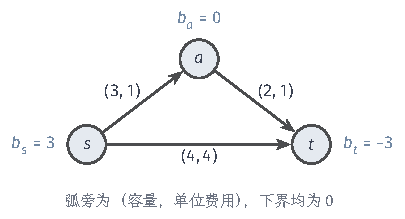
\includegraphics[width=68.527mm]{figures/01-basic-mathematics/04-graphs/tikz/c3-mcf-network/figure.pdf}
  \caption{三点最小费用流算例。$s$供给$3$单位，$t$需求$3$单位，$a$只做中转；弧旁括号依次为容量与单位费用，下界均为$0$。绕行$s\to a\to t$的单位费用为$2$，低于直达弧的$4$，但绕行量受$a\to t$的容量$2$限制。本节后面的计算都在这个网络上进行。}
  \label{fig:graph-opt-mcf-network}
\end{figure}

这个网络有许多可行流。$3$单位全走直达弧，费用为$3\times4=12$；让$2$单位绕行、$1$单位直达，费用为$2\times(1+1)+1\times4=8$。按弧序$s\to a$、$a\to t$、$s\to t$把流量写成向量，前者为$(0,0,3)$，后者为$(2,2,1)$。后面将证明$8$就是最小费用。

\paragraph{下界平移}
带正下界的弧在建模中很常见，例如合同规定某条线路至少运多少。处理办法是先把下界部分“预先送出”，再对剩余部分求解。令$x_{i,j}=\ell_{i,j}+y_{i,j}$，新变量满足$0\leq y_{i,j}\leq u_{i,j}-\ell_{i,j}$。预先送出的下界流量已经使顶点$i$净流出$\sum_j\ell_{i,j}-\sum_j\ell_{j,i}$，代入守恒式，$\bm y$应满足的剩余供需为
\[
  b'_i=b_i-\sum_{j:\,(i,j)\in E}\ell_{i,j}+\sum_{j:\,(j,i)\in E}\ell_{j,i}.
\]
目标变为$\sum c_{i,j}y_{i,j}+\bm c^{\top}\bm\ell$，后一项与$\bm y$无关。两个问题的可行解通过$\bm x=\bm\ell+\bm y$一一对应，费用处处相差同一个常数，所以最优解也一一对应。

图~\ref{fig:graph-opt-mcf-lower-bound}把三点网络中$s\to t$的下界改为$1$。平移后这条弧的容量从$4$变为$3$，同时$s$的剩余供给从$3$降为$2$，$t$的剩余需求从$3$降为$2$。如果只把容量减去下界而不修改供需，平移后的问题仍要求$s$送出$3$单位，下界那一单位就被重复计算了。新问题的最优解是$\bm y=(2,2,0)$，费用为$4$；加回常数$c_{s,t}\ell_{s,t}=4$，得到原问题的最优流$\bm x=(2,2,1)$与费用$8$。

\begin{figure}[!htb]
  \centering
  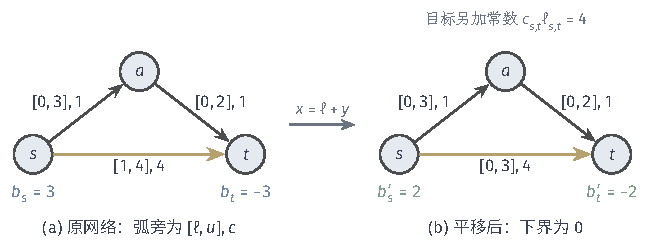
\includegraphics[width=109.767mm]{figures/01-basic-mathematics/04-graphs/tikz/c3-mcf-lower-bound-shift/figure.pdf}
  \caption{下界平移。(a)中黄色弧$s\to t$的流量须在$[1,4]$内，弧旁依次为流量区间与单位费用。(b)令$x=\ell+y$后，该弧的区间变为$[0,3]$，$s$与$t$的供需同时各减少$1$单位（绿色），目标另加常数$4$。容量和供需必须一起修改，只改其一会重复或遗漏下界那一单位。}
  \label{fig:graph-opt-mcf-lower-bound}
\end{figure}

上下界相等的弧流量已经固定，平移后容量为零，可以先删去，只保留它对供需和常数的贡献。还原时把平移量加回流量、把常数加回费用即可。以下除非特别说明，都假定下界已平移为零，固定弧已删去。

\paragraph{最优解的存在}
在有限上下界下，可行流集合由有限个线性等式与闭区间约束确定，是$\mathbb R^{a}$中的闭有界集，其中$a=|E|$。总费用是$\bm x$的线性函数，因而连续。由闭有界集上的极值定理~\ref{thm:multivariable-extreme-value}，只要可行流存在，最小费用一定能取到。可行流是否存在要另外判断，后文网络单纯形法的第一阶段就承担这一任务。

若允许某些弧的容量为无穷，可行集不再有界，最小值可能不存在。设可行流$\bm x$的残量网络（下一小节定义）中有一个负费用环，环上每条残量弧的剩余容量都是无穷，那么沿这个环可以推送任意多的流量，每推一单位都减少同样的正费用，总费用没有下界。本节主线只讨论有限容量。

还有一类常见问题：在源汇网络中先尽量多送，再在全部最大流中挑费用最低的，称为最小费用最大流。它分两步化成本节的问题：先用第~\ref{sec:graph-max-flow}节的方法求出最大流值$v^\star$，再令$b_s=v^\star$、$b_t=-v^\star$、其余$b_i=0$，求最小费用流。

\subsection{最优性条件}
\label{sec:graph-opt-mcf-optimality}

拿到一个可行流后，怎样判断它是否已经最便宜？逐一比较全部可行流行不通。第~\ref{sec:graph-max-flow}节判断最大流时，用残量网络把问题化成了“能否找到一条增广路径”。本小节沿用这一思路：先用残量网络描述所有保持供需的调整，再说明费用能否下降取决于其中是否有负费用环，最后借助节点势把环条件改写成逐弧可查的不等式。

\paragraph{残量网络与负费用环}
给定可行流$\bm x$。对每条原弧$(i,j)$，若$x_{i,j}<u_{i,j}$，建立正向残量弧$i\to j$，剩余容量为$u_{i,j}-x_{i,j}$，费用为$c_{i,j}$，表示再追加一单位要多付$c_{i,j}$；若$x_{i,j}>\ell_{i,j}$，建立反向残量弧$j\to i$，剩余容量为$x_{i,j}-\ell_{i,j}$，费用为$-c_{i,j}$，表示撤回一单位可以省下$c_{i,j}$。这与第~\ref{sec:graph-max-flow}节的残量网络相同，只是每条残量弧多带一个费用。原网络同时有$i\to j$与$j\to i$两条弧时，各自的残量弧要记住来自哪条原弧，不能合并成一个量。

沿残量网络中的有向环$C$推送$\theta>0$单位，是指对环上每条残量弧调整它的来源原弧：正向残量弧对应的原弧流量加$\theta$，反向残量弧对应的原弧流量减$\theta$。环上每个顶点恰有一条环弧进入、一条环弧离开，调整前后它的净流出不变，所以供需仍然满足；只要$\theta$不超过环上的最小剩余容量，上下界也仍然满足。总费用的改变量是$\theta\,c(C)$，其中$c(C)$是环上残量费用之和。于是，若$c(C)<0$，取正步长就能严格降低费用，当前流不是最优。

图~\ref{fig:graph-opt-mcf-residual-cycle}从全部走直达弧的可行流出发。残量网络中，$s\to a$与$a\to t$两条正向残量弧各费$1$，直达弧的反向残量弧$t\to s$费$-4$，三者构成费用为$1+1-4=-2$的环，剩余容量为$\min\{3,2,3\}=2$。沿这个环推送$2$单位，相当于把$2$单位从直达改为绕行，费用从$12$降为$12-2\times2=8$。

\begin{figure}[!htb]
  \centering
  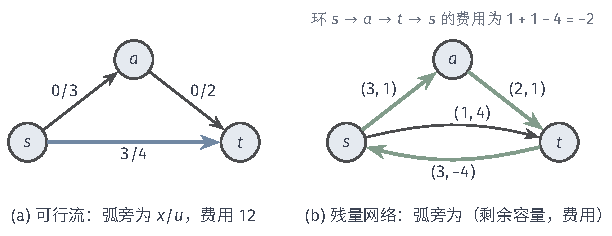
\includegraphics[width=103.579mm]{figures/01-basic-mathematics/04-graphs/tikz/c3-mcf-residual-cycle/figure.pdf}
  \caption{残量网络中的负费用环。(a)全部$3$单位走直达弧的可行流，弧旁为流量与容量。(b)它的残量网络，弧旁为剩余容量与费用；直达弧同时产生可追加$1$单位的正向残量弧和可撤回$3$单位、费用$-4$的反向残量弧$t\to s$。绿色环的费用为$-2$，沿它推送$2$单位使总费用降低$4$。}
  \label{fig:graph-opt-mcf-residual-cycle}
\end{figure}

\paragraph{环分解与最优性判据}
负费用环使费用可以下降。反过来，若残量网络中没有负费用环，是否就不存在更便宜的可行流？为此要说明：任何一个可行流与当前流之差，都能拆成残量网络中若干个环的叠加。

\begin{theorem}[负费用环判据]
\label{thm:graph-opt-negative-cycle}
可行流$\bm x$是最小费用流，当且仅当它的残量网络中不存在费用为负的有向环。
\end{theorem}

\begin{proof}
必要性已由上面的推送论证给出，下证充分性。任取可行流$\bm x'$，令$\bm d=\bm x'-\bm x$。两个流满足同一组供需，所以$\bm d$在每个顶点的净流出为零。逐条考察原弧$(i,j)$：若$d_{i,j}>0$，则$x_{i,j}<x'_{i,j}\leq u_{i,j}$，正向残量弧存在且剩余容量至少为$d_{i,j}$，在它上面放$d_{i,j}$；若$d_{i,j}<0$，则$x_{i,j}>x'_{i,j}\geq\ell_{i,j}$，反向残量弧存在，在它上面放$-d_{i,j}$。这样得到残量弧上的一组非负数$\bm g$，它在每个顶点的流入等于流出，并且按残量费用加权的总和等于$\sum_{(i,j)}c_{i,j}d_{i,j}=\bm c^{\top}\bm x'-\bm c^{\top}\bm x$。

接着把$\bm g$拆成环。若$\bm g\neq\bm 0$，从任一取正值的残量弧出发，沿正值弧前进：每到达一个顶点，它的流入为正，由流入等于流出，必有一条正值出弧可走。顶点只有有限个，前进中必然首次回到某个走过的顶点，由此截出一个有向环$C_1$。令$\lambda_1>0$为$\bm g$在$C_1$上的最小值，从环上各弧减去$\lambda_1$，剩余部分仍然非负且守恒，而取正值的弧至少少了一条。重复有限次，得到
\[
  \bm c^{\top}\bm x'-\bm c^{\top}\bm x=\sum_k\lambda_k\,c(C_k),\qquad\lambda_k>0.
\]
每个$C_k$都由残量弧组成。残量网络中没有负费用环时，右边每项非负，$\bm x'$不比$\bm x$便宜。
\end{proof}

判据回答的是怎样识别最优流，并不断言最优流唯一：若残量网络中有费用为零的环，沿它推送就得到另一个同费用的最优流。判据本身也不是完整的算法。反复寻找负费用环并沿它推送是一种自然的想法，但找哪个环、推多少、何时停止都要另行规定；下面的网络单纯形法给出一种具体的组织方式。

\paragraph{节点势与约化费用}
环判据要求检查所有的环，环的个数可能随图的规模指数增长。为了把它变成逐弧检查，给每个顶点$i$配一个实数$\pi_i$，称为\term{节点势}（node potential），并定义弧$(i,j)$的\term{约化费用}（reduced cost）
\begin{equation}
  \bar c_{i,j}=c_{i,j}-\pi_i+\pi_j.
  \label{eq:graph-opt-reduced-cost}
\end{equation}
残量弧使用同一公式：反向残量弧$j\to i$的费用为$-c_{i,j}$，约化费用为$-c_{i,j}-\pi_j+\pi_i=-\bar c_{i,j}$。

沿任一有向环把约化费用相加，每个顶点的势在离开它的弧上以$-\pi$出现一次、在进入它的弧上以$+\pi$出现一次，两两相消，所以环的约化费用之和等于原费用之和。因此，若能找到一组势，使所有残量弧的约化费用都非负，残量网络就没有负费用环。

反过来，残量网络没有负费用环时，这样的势一定存在。加入一个虚拟顶点$r$，从$r$向每个顶点连一条费用为零的弧。新弧都从$r$出发，没有弧进入$r$，所以新图的环都不经过$r$，仍然没有负环。由第~\ref{sec:graph-shortest-paths}节允许负边长的最短路结论，$r$到每个顶点$i$的最短距离$d_i$都是有限值（且$d_i\leq0$），并且对每条残量弧$i\to j$及其费用$c'$满足距离不等式$d_j\leq d_i+c'$。取$\pi_i=-d_i$，即得
\[
  c'-\pi_i+\pi_j=c'+d_i-d_j\geq0.
\]
所以“残量网络没有负费用环”与“存在使全部残量弧约化费用非负的势”等价，而后者只需逐弧检查。实际计算时可以用Bellman--Ford算法求$d_i$；若算法报告负环，就得到一个可以推送的负费用环。

\paragraph{逐弧最优性证书}
残量弧是否存在取决于原弧流量的位置，所以“全部残量弧的约化费用非负”可以翻译成原弧上的条件。弧$(i,j)$在下界时只有正向残量弧，要求$\bar c_{i,j}\geq0$；在上界时只有反向残量弧，要求$-\bar c_{i,j}\geq0$，即$\bar c_{i,j}\leq0$；严格位于两界之间时两条残量弧都存在，要求$\bar c_{i,j}=0$。下面的定理直接验证这组条件足以保证最优，不必再经过环分解。

\begin{theorem}[节点势最优性证书]
\label{thm:graph-opt-potential-certificate}
设固定弧已删去，$\bm x$是可行流，$\bm\pi$是一组节点势。若对每条弧$(i,j)$都有
\begin{equation}
  \bar c_{i,j}\ \begin{cases}
    \geq0, & x_{i,j}=\ell_{i,j},\\
    \leq0, & x_{i,j}=u_{i,j},\\
    =0, & \ell_{i,j}<x_{i,j}<u_{i,j},
  \end{cases}
  \label{eq:graph-opt-mcf-certificate}
\end{equation}
则$\bm x$是最小费用流。
\end{theorem}

\begin{proof}
任取可行流$\bm x'$。把$c_{i,j}=\bar c_{i,j}+\pi_i-\pi_j$代入费用差，
\[
  \bm c^{\top}(\bm x'-\bm x)=\sum_{(i,j)\in E}\bar c_{i,j}(x'_{i,j}-x_{i,j})+\sum_{(i,j)\in E}(\pi_i-\pi_j)(x'_{i,j}-x_{i,j}).
\]
第二个和按顶点重新归组，等于对每个$i$把$\pi_i$乘以顶点$i$在$\bm x'$与$\bm x$下净流出之差再求和；两个流满足同一组供需，这些差全为零。第一个和逐项非负：若$x_{i,j}=\ell_{i,j}$，则$x'_{i,j}-x_{i,j}\geq0$且$\bar c_{i,j}\geq0$；若$x_{i,j}=u_{i,j}$，则$x'_{i,j}-x_{i,j}\leq0$且$\bar c_{i,j}\leq0$；其余情形$\bar c_{i,j}=0$。所以$\bm c^{\top}\bm x'\geq\bm c^{\top}\bm x$。
\end{proof}

删去固定弧是为了避免$\ell_{i,j}=u_{i,j}$时前两个条件同时出现。条件~\eqref{eq:graph-opt-mcf-certificate}在线性规划中称为互补松弛条件，这里只用守恒式和每条弧允许的变化方向就完成了证明。流量$\bm x$与势$\bm\pi$合在一起构成一份证书：检查者核对可行性和每条弧上的一个符号，就能确认最优性，不必相信求解过程。回到三点网络，流$(2,2,1)$配上势$(\pi_s,\pi_a,\pi_t)=(4,3,0)$时，$s\to a$与$s\to t$都在两界之间，约化费用分别为$1-4+3=0$与$4-4+0=0$；$a\to t$在上界，约化费用为$1-3+0=-2\leq0$。三条弧都满足条件，所以费用$8$最小。

\subsection{网络单纯形法}
\label{sec:graph-opt-network-simplex}

定理~\ref{thm:graph-opt-potential-certificate}说明了停止时应该看到什么：一个可行流和一组势，逐弧满足符号条件。网络单纯形法始终保持流可行，并用一棵生成树确定势：树弧的约化费用被要求为零，由此解出势；再检查非树弧，若全部满足证书就停止，否则沿一个环改进流量。本小节以可行树基为算法状态，依次说明它的表示、第一个可行树基的构造、势的计算、环上的调整与状态更新，以及防止循环的选弧规则，最后用三点网络完整演示。

\paragraph{树基表示}
设下界已平移为零、固定弧已删去，并暂设底层无向图连通，即忽略弧的方向后连通。把弧集分成三部分：树弧集$T$，忽略方向后构成一棵生成树；取下界的非树弧集$L$；取上界的非树弧集$U$。三元组$(T,L,U)$称为一个\term{树基}（spanning tree basis）。非树弧的流量由它所在的集合直接给出，树弧的流量由守恒式决定。生成树总有叶子，叶子$v$只关联一条树弧，$v$的守恒式中其余各项（$b_v$与非树弧流量）都已知，于是解出这条树弧的流量；删去这个叶子及其树弧，把求出的流量计入相邻顶点的剩余供需，再对剩下的树重复，直到树弧全部求出。若求得的树弧流量都在上下界内，就称$(T,L,U)$为可行树基。

这里有两点容易误解。第一，树弧的流量允许恰好等于上界或下界；一条弧是否属于$T$取决于它在树中的位置，而不是流量是否严格在界内。第二，树不要求所有弧都朝向某个根，弧的方向只决定它在守恒式中取正号还是负号。

图~\ref{fig:graph-opt-ns-tree-basis}(a)是一个五点例子，供需为$b=(4,0,-2,1,-3)$，非树弧$1\to4$在上界、流量为$2$，$2\to5$在下界、流量为$0$。叶子$1$的守恒式为$x_{1,2}+x_{1,4}=4$，得$x_{1,2}=2$；叶子$4$的守恒式为$x_{4,3}-x_{1,4}=1$，得$x_{4,3}=3$，恰好等于这条树弧的容量；叶子$5$的守恒式为$-(x_{3,5}+x_{2,5})=-3$，得$x_{3,5}=3$。删去这三个叶子后，顶点$2$成为叶子，由$x_{2,3}+x_{2,5}-x_{1,2}=0$得$x_{2,3}=2$。最后剩下的顶点$3$的守恒式$x_{3,5}-x_{2,3}-x_{4,3}=3-2-3=-2$自动成立，因为全部供需之和为零。

\begin{figure*}[!htb]
  \centering
  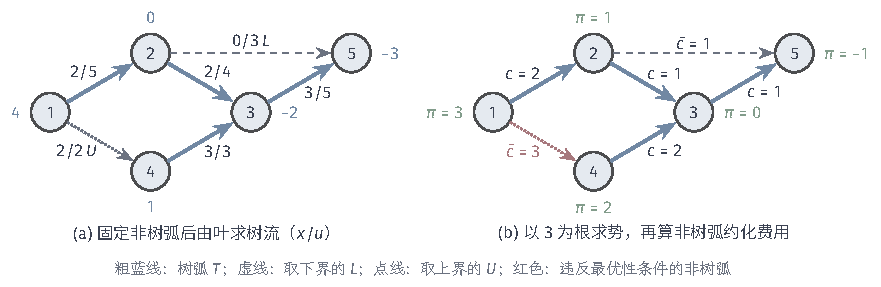
\includegraphics[width=149.144mm]{figures/01-basic-mathematics/04-graphs/tikz/c3-ns-tree-basis/figure.pdf}
  \caption{五点网络上的树基。粗蓝弧为树弧，虚线弧取下界，点线弧取上界。(a)顶点旁为供需量，弧旁为流量与容量；固定两条非树弧后，从叶子$1,4,5$开始逐个用守恒式求出树弧流量，树弧$4\to3$恰在上界仍属于树。(b)弧旁为单位费用或约化费用，绿色为以顶点$3$为根求出的节点势；树弧约化费用均为零，非树弧$1\to4$在上界却有$\bar c=3>0$（红色），违反最优性条件。}
  \label{fig:graph-opt-ns-tree-basis}
\end{figure*}

树流为什么由树唯一确定，可以用关联矩阵说明。按第~\ref{sec:graph-representations}节的约定，关联矩阵$\bm B\in\mathbb R^{n\times a}$中弧$(i,j)$对应的列在第$i$行为$1$、第$j$行为$-1$，守恒式就是$\bm B\bm x=\bm b$。$\bm B$各行之和为零，删去根所在的一行不丢失信息，记剩下的矩阵为$\tilde{\bm B}$。树弧对应的列组成$(n-1)$阶方阵$\tilde{\bm B}_T$。按上面消去叶子的次序排列行与列，每消去一个叶子，它所在的行在剩余树弧列中只有一个非零元，所以$\tilde{\bm B}_T$经行列重排后是三角矩阵，对角元为$\pm1$，从而可逆。于是$\bm x_T=\tilde{\bm B}_T^{-1}(\tilde{\bm b}-\tilde{\bm B}_N\bm x_N)$唯一确定，其中$N=L\cup U$；供需与界都是整数时，树流也是整数。

底层无向图不连通时，在消去固定弧后的各弱连通分量中分别处理：每个分量内的剩余供需之和必须为零，否则问题不可行；孤立顶点没有任何弧，它的供需必须为零。另外，同一个流量可能对应不同的树基，例如树弧恰在界上时，它也可能作为非树弧出现在另一个树基中。后面的退化现象正来自这种区别。

\paragraph{初始可行树基}
任意选一棵生成树、令非树弧取下界，求得的树流未必满足上下界。例如在三点网络中取$T=\{s\to a,a\to t\}$、$s\to t$取下界，叶子$a$与$t$迫使$x_{a,t}=3$，超过容量$2$。因此第一个可行树基要专门构造。

在下界已平移为零的网络中，先令全部原弧流量为零，再增加一个人工根$r$：每个$b_i>0$的顶点连人工弧$i\to r$，流量为$b_i$；每个$b_i<0$的顶点连人工弧$r\to i$，流量为$-b_i$；$b_i=0$的顶点连人工弧$i\to r$，流量为零。人工弧的容量取总供给$\sum_{b_i>0}b_i$，足以容纳这些流量。人工弧构成以$r$为中心的星形生成树，每个原顶点的守恒式都由它唯一的人工弧满足，于是得到一个显式的可行树基。

第一阶段令原弧费用为零、人工弧单位费用为一，目标就是人工流的总量，用下面介绍的同一套入弧、环调整与防循环操作求解。若第一阶段最优值为零，人工弧全部空载，原弧上的流量满足原问题的全部约束；若最优值为正，原问题没有可行流，因为原问题的任何可行流配上全零人工流都会使第一阶段目标为零。这一判定不依赖人为选定的“很大的费用常数”。

第一阶段结束后，删去人工根和全部人工弧。原来的树弧中去掉人工弧，留下一个森林；在原图的每个弱连通分量内，用连接不同森林分量的原非树弧把它补成生成树。补入的弧保持原流量不变，它们本来就在上界或下界，作为树弧恰在界上是允许的。随后恢复原费用、重新计算节点势，并从所得的可行树基重新设置防循环所需的数据，进入第二阶段。

\paragraph{节点势的计算}
给定树基，令根的势为零，沿树逐条解方程$c_{i,j}-\pi_i+\pi_j=0$，使每条树弧的约化费用为零。沿树弧方向从已知的$\pi_i$走到$j$时取$\pi_j=\pi_i-c_{i,j}$，逆着树弧方向从已知的$\pi_j$走到$i$时取$\pi_i=\pi_j+c_{i,j}$。换一个根只让全部势同加一个常数，约化费用不变。树流由供需与非树弧的界状态决定，势则只由树的结构与费用决定，两者分别计算。

图~\ref{fig:graph-opt-ns-tree-basis}(b)以顶点$3$为根：逆着$2\to3$得$\pi_2=0+1=1$，再逆着$1\to2$得$\pi_1=1+2=3$；逆着$4\to3$得$\pi_4=0+2=2$；顺着$3\to5$得$\pi_5=0-1=-1$。随后计算非树弧的约化费用：$2\to5$为$3-1+(-1)=1\geq0$，在下界，符合条件；$1\to4$为$4-3+2=3>0$，却在上界，违反条件。

树弧的约化费用都是零，无论流量位于何处都满足条件~\eqref{eq:graph-opt-mcf-certificate}。所以只要全部非树弧也满足条件，即$L$中的弧$\bar c\geq0$、$U$中的弧$\bar c\leq0$，当前流与势就构成最优性证书，算法停止。寻找违反条件的非树弧，称为定价。

\paragraph{入弧与环调整}
违反条件的非树弧有两类：$L$中$\bar c_{i,j}<0$的弧，应沿正向增加流量；$U$中$\bar c_{i,j}>0$的弧，应沿反向减少流量。选定这样一条入弧后，它与树上连接两端点的唯一路径构成一个环，称为\term{基本环}（fundamental cycle）。按入弧的调整方向给环定向：环上顺着定向经过的弧增加流量，逆着定向经过的弧减少流量。环上每个顶点一进一出，调整保持守恒。

推送一单位时，费用变化是环上各弧费用按增减取正负号之和。把每个$c$换成$\bar c+\pi_i-\pi_j$，势沿环相消，而树弧的约化费用为零，所以单位费用变化恰为入弧在调整方向上的约化费用：正向进入时为$\bar c_{i,j}<0$，反向进入时为$-\bar c_{i,j}<0$。

接着确定能推多远。对环上增加流量的弧计算$u-x$，对减少流量的弧计算$x-\ell$，入弧自身也参加比较，取最小值作为步长$\theta$。按$\theta$沿环更新后守恒仍然成立，上下界也都满足。$\theta>0$时费用严格下降$\theta|\bar c_{i,j}|$；$\theta=0$时流量不变，这种情形留到后面专门讨论。

\paragraph{出弧与状态更新}
达到步长$\theta$的弧称为阻塞弧，可能不止一条，按后述防循环规则从中选出一条。若选中的是树弧，它离开树，按它到达的是下界还是上界归入$L$或$U$，入弧则加入$T$。被删去的弧位于基本环上，删去后树仍然连通且无环，新的$T$仍是生成树。势需要更新：最简单的做法是沿新树从根重新计算一遍，便于逐步复核。更省的做法只调整一部分顶点：删去出弧后树分成两块，只有不含根的那一块的势改变，且同加或同减入弧的约化费用。

若选中的是入弧自身，说明它先到达了另一端的界，便从$L$转入$U$或从$U$转入$L$，树和势都不变。这种\emph{界翻转}同样是合法的一次迭代，所以不能把每一轮都描述为两条不同的弧互相交换。

\begin{algorithm}[网络单纯形法]
\label{alg:graph-opt-network-simplex}
输入：有限有向网络，供需$b_i$，有限上下界与单位费用。输出：最优流$\bm x$、费用与节点势$\bm\pi$，或“不可行”的结论。状态：树基$(T,L,U)$、各弧流量（含扰动系数）、树的父顶点与深度、节点势。
\begin{enumerate}
  \item 平移下界、删去固定弧；在每个弱连通分量内检查供需之和为零。
  \item 第一阶段：增加人工根与人工弧，取星形可行树基，原弧费用为零、人工弧费用为一，并按当前树基设置防循环数据。
  \item 计算节点势与非树弧的约化费用；若没有违反条件的非树弧，转第6步。
  \item 选一条违反条件的入弧，构造基本环，比较环上各弧（含入弧）的剩余量得到步长$\theta$，按防循环规则选出阻塞弧。
  \item 沿环更新流量；若出弧是树弧，作树弧交换，否则作界翻转。回到第3步。
  \item 第一阶段停止时，若人工流总量为正，报告不可行；否则删去人工结构，补成原网络的可行树基，恢复原费用并重新设置防循环数据，以第二阶段身份回到第3步。第二阶段停止时，还原下界平移，返回流量、费用与节点势。
\end{enumerate}
\end{algorithm}

\paragraph{退化与防循环}
步长为零的迭代称为\term{退化换基}（degenerate pivot）。它发生在基本环上某条弧已经处在阻塞方向的界上时，通常就是恰在界上的树弧。图~\ref{fig:graph-opt-ns-degenerate}把三点网络中$s\to t$的容量改为$1$，从$T=\{s\to a,a\to t\}$、$U=\{s\to t\}$出发，流量为$(2,2,1)$，树弧$a\to t$已在上界。势为$(2,1,0)$，$s\to t$在上界而$\bar c_{s,t}=4-2+0=2>0$，应反向进入；基本环上$a\to t$要增加流量，剩余量为$0$，所以$\theta=0$。$a\to t$出基进入$U$，$s\to t$进入树，流量和费用都没变，树基却变了。在新树基下势为$(4,3,0)$，$\bar c_{a,t}=-2\leq0$，满足条件，算法停止。

\begin{figure}[!htb]
  \centering
  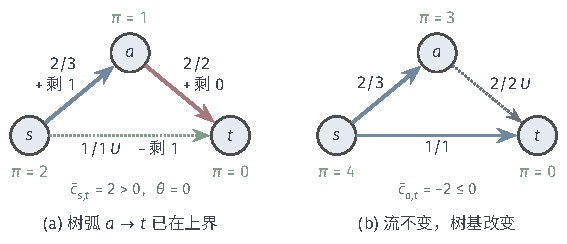
\includegraphics[width=96.054mm]{figures/01-basic-mathematics/04-graphs/tikz/c3-ns-degenerate/figure.pdf}
  \caption{退化换基。三点网络中$s\to t$的容量改为$1$，弧旁为流量与容量，“剩”为沿基本环调整方向的剩余量，绿色$\pi$为节点势。(a)入弧$s\to t$（绿色）在上界且约化费用为正，反向进入；树弧$a\to t$（红色）已在上界，剩余量为零，步长为零。(b)$a\to t$出基后流量与费用不变，新树基的势使全部非树弧满足最优性条件。}
  \label{fig:graph-opt-ns-degenerate}
\end{figure}

这个例子中的退化换基换来了一份最优性证书，但一般情形下，连续的零步长换基可能在若干个树基之间兜圈子，回到已经出现过的树基，费用始终不变，算法不再前进。因此，“费用不增加”本身不足以保证有限终止，阻塞弧有多条时选哪一条，必须写进算法。只取编号最小的弧不能排除循环，需要专门构造的规则。下面说明适用于有上下界弧的\term{词典序规则}（lexicographic rule）。

把上界写成等式$x_{i,j}+s_{i,j}=u_{i,j}$，$s_{i,j}\geq0$是上界松弛量。这样，每条弧有两个离界距离：$x_{i,j}-\ell_{i,j}$与$s_{i,j}$。非退化的情形是每条树弧的两个离界距离都为正，步长才一定为正。词典序规则用一个符号扰动人为地制造这种情形。在一个阶段开始时，把当前可行树基的树弧编号为$e_1,\ldots,e_{n-1}$，把$e_k$的流量改为$x_{e_k}+\sigma_k\varepsilon^k$：若$e_k$在上界取$\sigma_k=-1$，否则取$\sigma_k=+1$。供需随之改为扰动后流量所对应的净流出，并在整个阶段内保持不变；非树弧仍恰在界上。这里$\varepsilon$看作充分小的正数，每个量都表示成$(\text{常数},\varepsilon\text{的系数},\ldots,\varepsilon^{n-1}\text{的系数})$这样的向量，比较大小就是从常数项起按分量逐个比较，即词典序比较。于是每条树弧的两个离界距离在词典序下都严格为正。

每轮比较步长时，增加流量的树弧以向量$u-x(\varepsilon)$为候选，减少流量的树弧以$x(\varepsilon)-\ell$为候选，入弧以$(u-\ell,0,\ldots,0)$为候选，取词典序最小者作为步长$\theta(\varepsilon)$并让它出基。初始时各树弧的$\varepsilon$系数行是$\pm$单位向量，线性无关；每次换基，留下的树弧系数行加减出弧的系数行，入弧取出弧系数行的正负，这是可逆的行变换，界翻转则不改变系数行。所以各树弧的系数行始终线性无关，两条树弧的候选向量不会相等，入弧的候选向量与任一树弧也不会相等，词典序最小者唯一。更新后出弧恰好落在界上，其余树弧仍严格在界内，扰动后的问题始终非退化。

还原到基本环上，这个规则只在实际步长出现并列时起作用：比较并列阻塞弧的$\varepsilon$系数，选词典序最小的那条出基，实际流量仍按常数项更新。它为什么能防止循环，在下一小节的分析中说明。两个阶段各自从初始可行树基设置扰动：第一阶段从星形树基开始，第二阶段从清理人工结构后得到的树基重新开始。另一类常用规则要求维护所谓强可行树，它有自己的方向约定与初始化要求；第一阶段清理只保证得到普通的可行树基，不能据此断言原网络已经具有强可行树，这里不展开。

\paragraph{迭代算例}
回到图~\ref{fig:graph-opt-mcf-network}的三点网络，先做第一阶段。人工弧容量取总供给$3$，星形初始树为$s\to r$、$r\to t$、$a\to r$，流量依次为$3,3,0$，人工流总量为$6$，见图~\ref{fig:graph-opt-ns-artificial-start}(a)。按这个次序设置扰动，前两条树弧在上界，扰动后的流量为$3-\varepsilon$与$3-\varepsilon^2$，$a\to r$为$\varepsilon^3$。以$r$为根，第一阶段费用下的势为$(\pi_s,\pi_a,\pi_t,\pi_r)=(1,1,-1,0)$，非树弧$s\to t$与$a\to t$的约化费用都是$-2$。

\begin{figure*}[!htb]
  \centering
  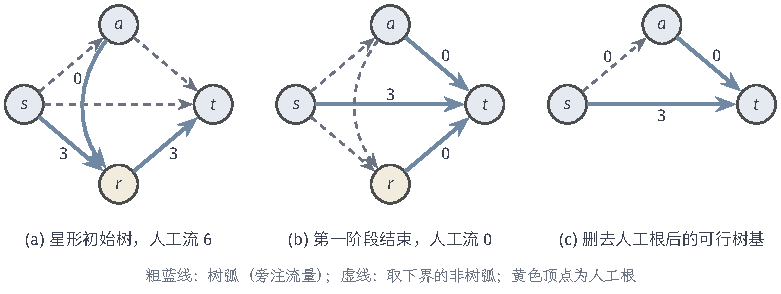
\includegraphics[width=132.186mm]{figures/01-basic-mathematics/04-graphs/tikz/c3-ns-artificial-start/figure.pdf}
  \caption{两阶段法的第一阶段。(a)增加人工根$r$（黄色），供给点、需求点和中转点分别用人工弧连向或连自$r$，得到显式可行的星形树，人工流总量为$6$。(b)两次换基后人工流降为零，原弧$s\to t$承担全部$3$单位，空载的人工弧$r\to t$仍在树中。(c)删去人工根和人工弧，剩下的树弧恰好构成原网络的生成树，作为第二阶段的初始可行树基。}
  \label{fig:graph-opt-ns-artificial-start}
\end{figure*}

选$s\to t$入弧。基本环上$s\to t$增加，$r\to t$与$s\to r$减少，剩余量依次为$4$、$3$、$3$，实际步长并列。两条并列弧的候选向量为$(3,0,-1,0)$与$(3,-1,0,0)$，后者词典序更小，所以$s\to r$出基。更新后$s\to t$承担$3$单位，人工流的常数部分已经为零。新势为$(-1,1,-1,0)$，$a\to t$的约化费用为$0-1+(-1)=-2$，再次入弧；这次$r\to t$与$a\to r$的剩余量都是$0$，是一次退化换基，比较$\varepsilon$系数后$a\to r$出基。此时全部非树弧满足条件，第一阶段最优值为零，见图~\ref{fig:graph-opt-ns-artificial-start}(b)。删去$r$后，树弧$s\to t$与$a\to t$已经构成原网络的生成树，$s\to a$在下界，这就是第二阶段的初始树基。

第二阶段从$T=\{s\to t,a\to t\}$、流量$(0,0,3)$开始，总费用为$12$。以$t$为根，逆着$s\to t$得$\pi_s=4$，逆着$a\to t$得$\pi_a=1$，势为$(4,1,0)$。非树弧$s\to a$在下界，约化费用为$1-4+1=-2<0$，选它正向入弧。基本环为$s\to a\to t$再逆着$s\to t$回到$s$：$s\to a$与$a\to t$增加，剩余量为$3$与$2$；$s\to t$减少，剩余量为$3$。步长$\theta=2$，由$a\to t$达到，费用下降$2\times2=4$。

$a\to t$到达上界，出基进入$U$，$s\to a$进入树。新流量为$(2,2,1)$，总费用为$8$。以$t$为根重新计算，$\pi_s=4$，顺着$s\to a$得$\pi_a=4-1=3$，势为$(4,3,0)$。唯一的非树弧$a\to t$在上界，约化费用为$1-3+0=-2\leq0$，满足条件，算法停止。这正是上一小节核对过的最优性证书。

再把$s\to a$的容量改为$1$，从同一初始树基出发。势与约化费用都不变，$s\to a$仍正向入弧，但三条弧的剩余量变为$1$、$2$、$3$，步长为$1$，由入弧自身达到。于是作界翻转：$s\to a$从$L$转入$U$，树不变，流量为$(1,1,2)$，费用为$10$。势仍为$(4,1,0)$，$s\to a$在上界，约化费用$-2\leq0$；没有其他非树弧，算法停止。逐项核对：$s$的净流出$1+2=3$，$a$的净流出$1-1=0$，$t$的净流出$-1-2=-3$，各弧流量都在界内。

图~\ref{fig:graph-opt-ns-pivots}把两种情形并排比较。两者从同一个树基、同一条入弧出发，只因入弧容量不同，阻塞弧一次是树弧、一次是入弧自身，分别对应树弧交换与界翻转。

\begin{figure*}[!htb]
  \centering
  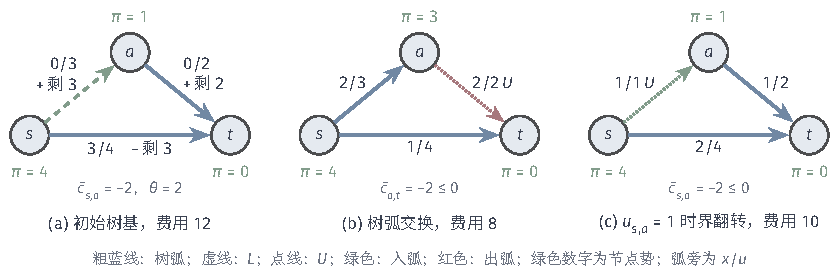
\includegraphics[width=142.053mm]{figures/01-basic-mathematics/04-graphs/tikz/c3-ns-pivots/figure.pdf}
  \caption{第二阶段的两种迭代。弧旁为流量与容量，“$+$剩”“$-$剩”为沿基本环增加或减少流量时的剩余量，$\pi$为节点势。(a)初始树基中$s\to a$的约化费用为$-2$，沿基本环最多推送$2$单位。(b)阻塞弧是树弧$a\to t$，它出基进入$U$，费用由$12$降为$8$。(c)若$s\to a$容量为$1$，入弧自身先到上界，树不变，费用降为$10$。两种结局中非树弧的约化费用都满足符号条件。}
  \label{fig:graph-opt-ns-pivots}
\end{figure*}

\subsection{算法分析与结果检验}
\label{sec:graph-opt-ns-analysis}

前面逐步说明了网络单纯形法的各个操作，本小节把它们合起来，回答三个问题：每轮迭代是否保持可行并改进费用，算法是否一定停止，停止时得到的是什么、要花多少计算。

\paragraph{可行性与费用变化}
每轮迭代沿基本环调整流量，环上每个顶点一进一出，各顶点的净流出不变；步长取环上各弧剩余量的最小值，所以调整后上下界仍然满足。树弧交换后新的$T$仍是生成树，出弧落在它所到达的界上，被正确归入$L$或$U$；界翻转只改变入弧的界状态。因此，每轮结束时都得到一个可行树基。费用的变化等于步长乘以入弧在调整方向上的约化费用，后者为负：步长为正时费用严格下降，步长为零时费用不变而树基改变。

\paragraph{有限终止}
仅凭费用不增不能推出有限终止，因为零步长的换基可能循环。词典序规则补上了这一缺口。在一个阶段内，扰动后的供需固定不变，扰动后的流量由树基$(T,L,U)$唯一确定，所以扰动后的费用（一个关于$\varepsilon$的多项式）是树基的函数。扰动后的问题非退化，每轮的步长$\theta(\varepsilon)$在词典序下严格为正，扰动后的费用便在词典序下严格下降，已经出现过的树基不可能再出现。可能的树基只有有限个：$T$是有限多棵生成树之一，每条非树弧只有两种界状态。所以每个阶段都在有限轮后停止。

停止时全部非树弧满足符号条件，树弧约化费用为零，由定理~\ref{thm:graph-opt-potential-certificate}，当前流在本阶段的费用下最优。对第一阶段，这给出可行性的判定；对第二阶段，这给出原问题的最优流。以上论证都假设精确运算。

\paragraph{单轮开销}
设顶点数为$n$，弧数为$a$。朴素实现每轮扫描全部非树弧计算约化费用，需要$O(a)$次运算；为树记录父顶点与深度后，从入弧两端沿父指针上溯到最近公共祖先即可找出基本环，并沿环比较剩余量、更新流量，都是$O(n)$；沿新树重新计算势也是$O(n)$。所以每轮为$O(n+a)$次运算，只扫描部分弧的定价策略可以降低这一项。总开销还取决于迭代轮数，其中包括退化换基。上面的有限性论证只给出与树基个数相当的上界，不能从每轮简单推出总运算量具有统一的多项式界；本书也不据此断言网络单纯形法一定快于专门的最大流或指派算法。

\paragraph{结果检验}
输出须回到原始问题检查：先把下界平移量加回流量，核对每个顶点的净流出等于原始$b_i$、每条弧满足原始上下界，再按原始费用重算目标值，并确认它等于平移后问题的费用加上常数$\bm c^{\top}\bm\ell$。最优性则逐弧核对势条件~\eqref{eq:graph-opt-mcf-certificate}。浮点实现中，守恒误差、界约束误差与约化费用的符号都只能在容差内判断，应分别报告；近似满足的条件说明结果接近最优，不能直接当作精确证书。

\paragraph{与其他问题的关系}
最大流与最小费用流使用同一种残量网络，但改进方式不同：最大流沿源汇之间的增广路径增加输送量，最小费用流在供需固定时沿环调整流量以减少费用。下一节的匹配可以写成单位容量的最大流，第~\ref{sec:graph-assignment}节的指派则可以写成单位容量的最小费用流。尽管如此，后面两节仍分别介绍专门的增广算法：一般模型说明问题之间可以互相转写，专门算法则利用二部配对的结构，状态更简单，开销也有更直接的界。
